\chapter{Evaluation}\label{ch:evaluation}
Parameters of models

\subsection{\eigendocs}\label{subsec:evaluation-eigendocs}

\textcolor{red}{TODO: compare preprocessing results}


% preprocessed images
\begin{figure}[htp] % htp = hier (h), top (t), oder auf einer eigenen Seite (p).
    \centering
    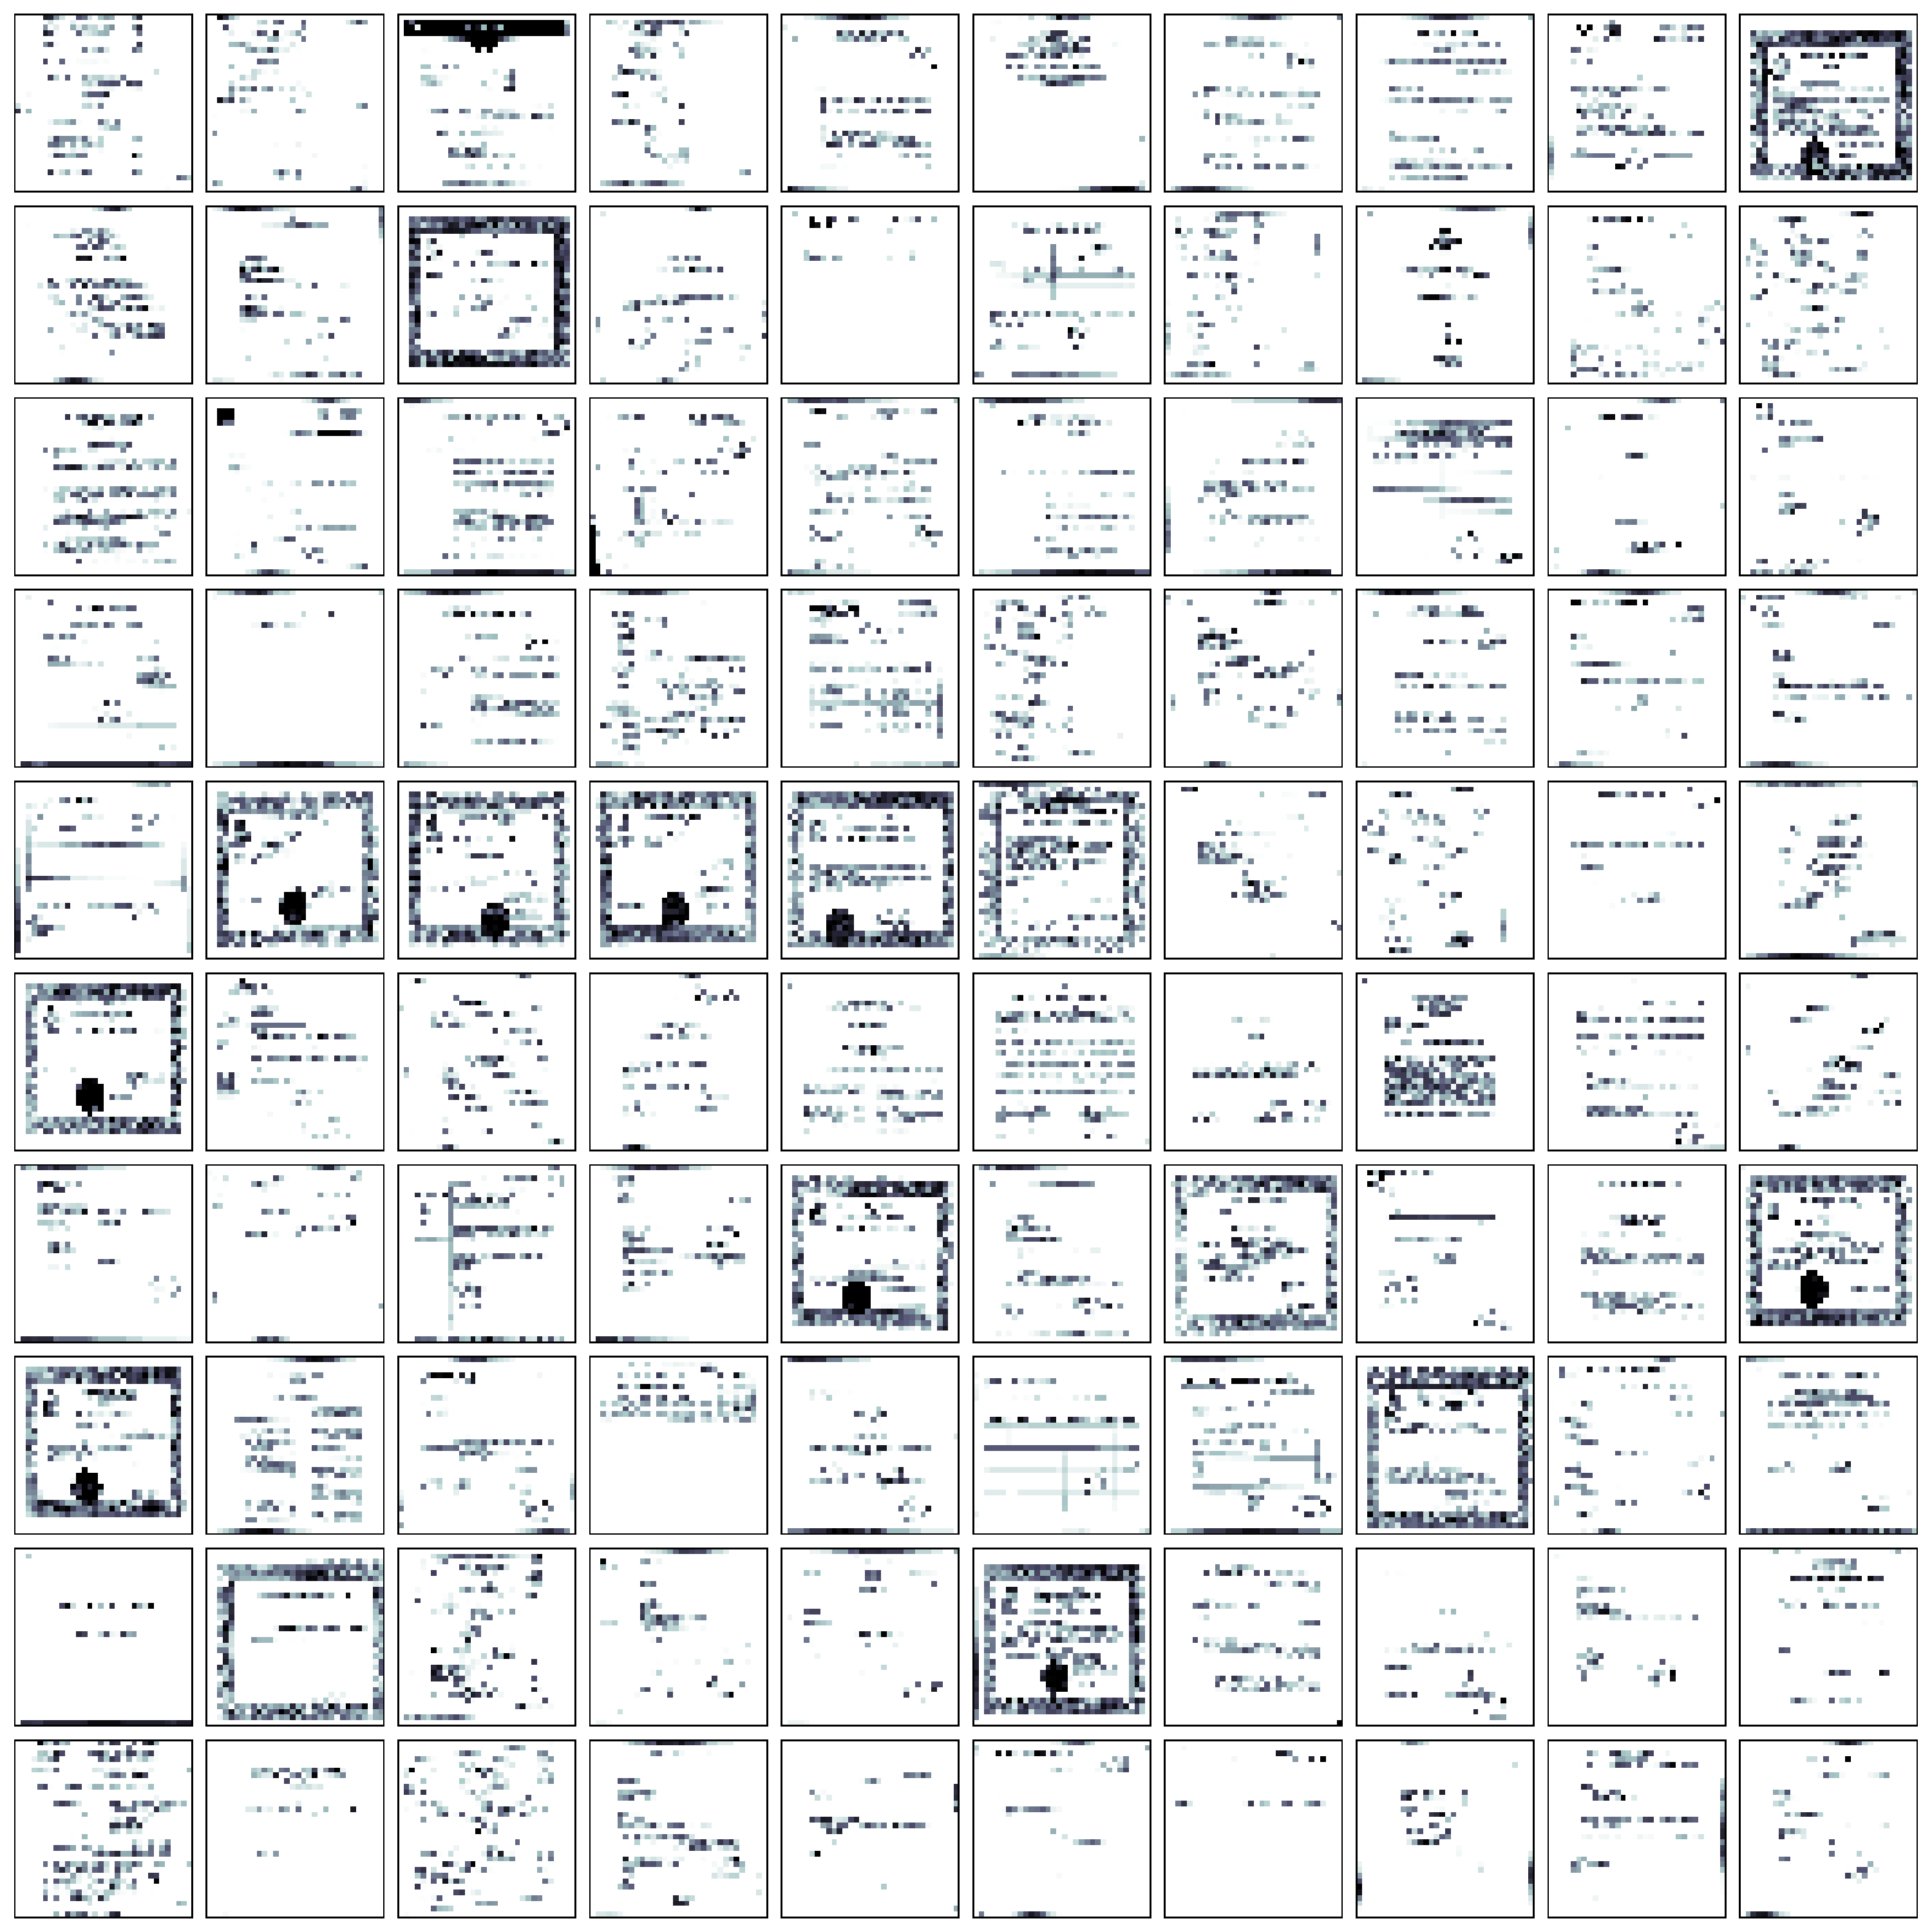
\includegraphics[width=0.5\textwidth]{images/OPTICS/32x32/preprocessed_docs.pdf}
    \caption{The first 100 preprocessed documents of the dataset.
    They were preprocessed in order to have the same characteristics as the images used in \cite{OPTICS1999}.
    The images were preprocessed as discussed in \autoref{pt:32} to 32x32 greyscale pixels, which drastically reduced the quality of the images.
    }
    \label{fig:preprocessed_docs_32x32}
\end{figure}

\begin{figure}[htp] % htp = hier (h), top (t), oder auf einer eigenen Seite (p).
    \centering
    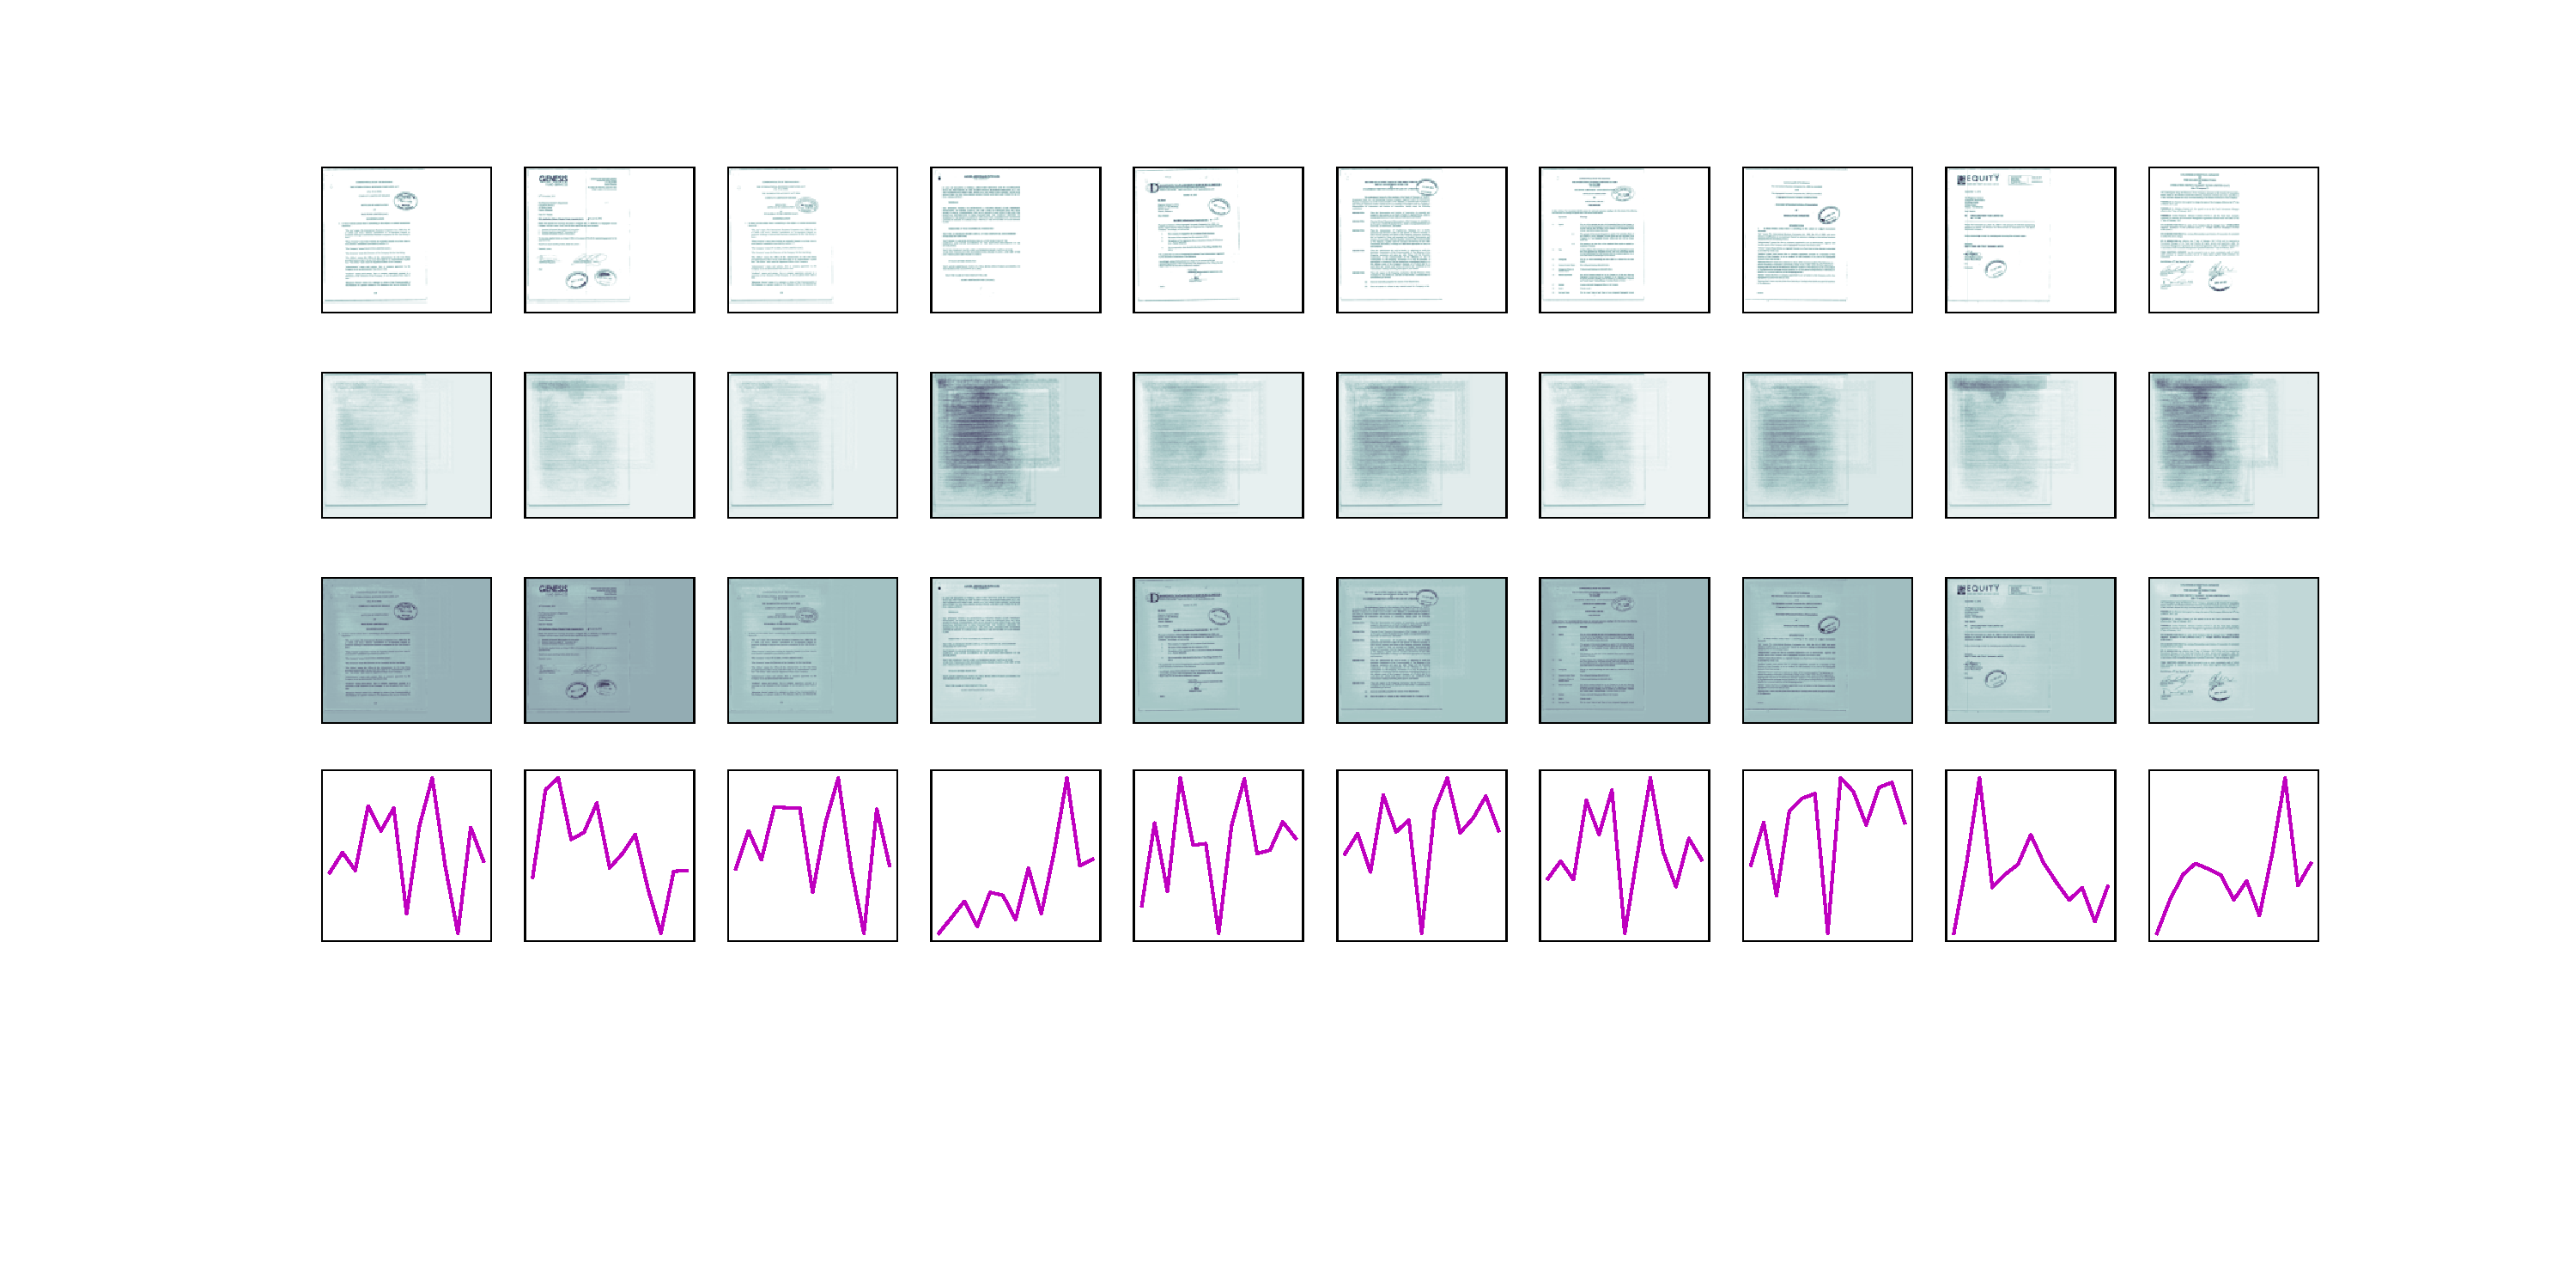
\includegraphics[width=0.7\textwidth]{images/Eigendocs/transformation/eigendocs_13dims.pdf}
    \caption{The first 10 preprocessed documents of the dataset.
    The original images are displayed in the first row.
    The second row shows the reconstructed images using the compressed images from the fourth row.
    The third row shows the reconstruction error, i.e. the difference between the reconstructed and the original image.
    The fourth row shows them in their compressed 2x2 greyscale form as discussed in \autoref{pt:eigendocs}.
    The last row presents the greyscale values of the compressed image as a line.
    }
    \label{fig:preprocessed_docs_eigendocs}
\end{figure}


% OPTIC cluster results
\begin{figure}%
    \centering
    \subfloat[\centering The clusters identified by \ac{optics} of the documents preprocessed according to \autoref{pt:32}.]{{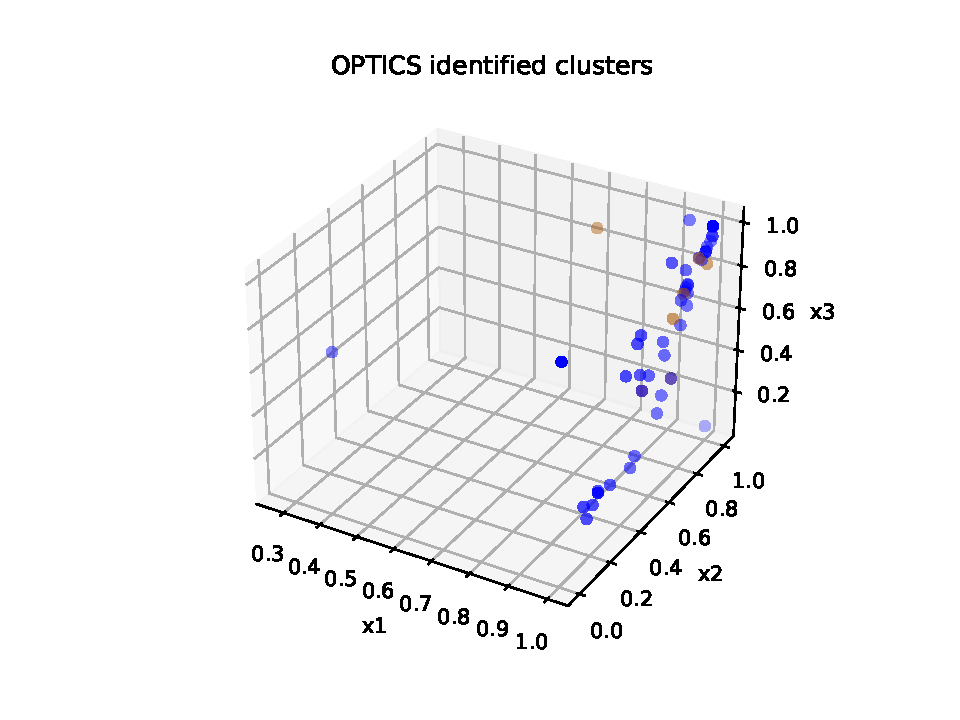
\includegraphics[width=5cm]{images/OPTICS/32x32/OPTICS_cluster_32x32.pdf} }}%
    \qquad
    \subfloat[\centering The clusters identified by \ac{optics} of the documents preprocessed according to \autoref{pt:eigendocs}.]{{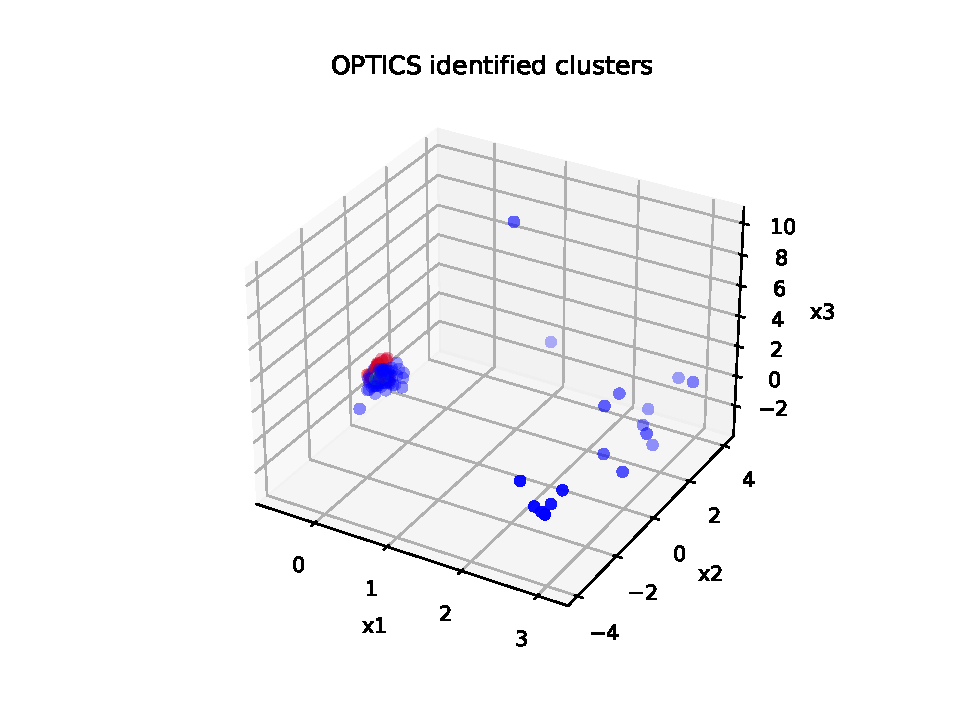
\includegraphics[width=5cm]{images/OPTICS/eigendocs/OPTICS_cluster_eigendocs.pdf} }}%
    \caption{The clusters were extracted from the respective reachability plot in \autoref{fig:reachability_plots}.
    The blue points are noise points, whereas any other colour denotes a cluster.}%
    \label{fig:optics_cluster}%
\end{figure}


\section{analysis/ comparison of models}\label{sec:evaluation-models}
difference query responses for different models?
any images which produce unusual results?

\section{Evaluation of the performance}\label{sec:evaluation-performance}

\subsection{Fahnder clustern}\label{subsec:evaluation-metric1}

\subsection{Fahnder bewerten Resultate (image matrix)}\label{subsec:evaluation-metric2}

\section{Evaluation of the usability}\label{sec:evaluation-usability}

\subsection{Metrics}\label{subsec:evaluation-metrics}